\section{Main Results}
\label{sec:main-results}

%\yry{search realize and change to realize; introduce the realize symbol in main text.}
Given the function and pipeline models, we now present our main results, on whether a function $f$ can be realized by a pipeline $p$.

To simplify the reading of our results, we put only the definitions and main results in the main text. The proofs of the results are in the appendix. To make it easier to follow the symbols, we collect key symbols in Table I for reference.

\begin{table}
\centering
\begin{tabular}{| l | l |}
  \hline
  \textbf{Symbol} & \textbf{Definition}\\
  \hline
  \hline
  \multicolumn{2}{|l|}{\textbf{Routing function symbols}} \\
  \hline
  $f$ & Routing function\\
  $\mathcal{F}$ & Routing function space\\
  $m_i$ & Packet match field\\
  $\mathcal{M}$ & Set of $\forall\ m_i$\\
  $dom(M)$ & Domain of valid values of $M$\\
  $\mathcal{R}$ & Set of $\forall$ valid routing actions\\ 
  \hline
  \hline
  \multicolumn{2}{|l|}{\textbf{Pipeline symbols}} \\
  \hline
  $p$ & Pipeline\\
  $\mathcal{P}$ & Pipeline function space\\
  $t_i$ & Pipeline table\\
  $r(t_i)$ & $t_i$'s output register\\
  $bits(r(t_i))$ & $t_i$'s output register bit length\\
  $I(t_i)$ & $t_i$'s table inputs\\
  $maxrules(t_i)$ & Maximum $\#$ of rules $t_i$ can contain\\
  \hline
\end{tabular}
\vspace{2mm}
\label{tbl:sym-table}
\caption{Symbol table listing notation in our main results.}
\end{table}

\subsection{Overview}
%---\yry{we denote xxx when f can be realized by p}--
A main challenge in developing a systemic method to verify whether a routing function $f$ can be realized by a pipeline $p$, which we denote as $f \rightrightharpoons p$, is that routing functions and pipelines are represented differently and both types of representations can have substantial complexities and variations. Consider each routing function $f$ as a point in a functional space $\mathcal{F}$, and each pipeline $p$ as a point in functional space $\mathcal{P}$. 

Our main contribution is the introduction of a novel, unifying, normalization functional space $\mathcal{C}$ called the characteristic functions space. Each routing function $f$ is mapped by the mapping $\tau$ to a characteristic function $\tau(f) \in \mathcal{C}$, characterizing the computational load of $f$. Each pipeline $p$, on the other hand, is mapped to a set $\kappa(p) \subset \mathcal{C}$ of characteristic functions, representing the set of computational capabilities of the pipeline. 
Fig~\ref{fig:function-spaces} illustrates the mapping structure.

%The main structure of our main result is that we can then define a third, ordered space , the space of $\forall\ c$ and produce mappings from $\mathcal{F}$ and $\mathcal{P}$ to $\mathcal{C}$ and $2^\mathcal{C}$ which we denote $\tau$ and $\kappa$ respectively. These three spaces $\mathcal{F}$, $\mathcal{P}$ and $\mathcal{C}$ and the mappings between them in are shown in Fig~\ref{fig:function-spaces}.

\begin{figure}[tbh]
    \centering
    \vspace{-1mm}
    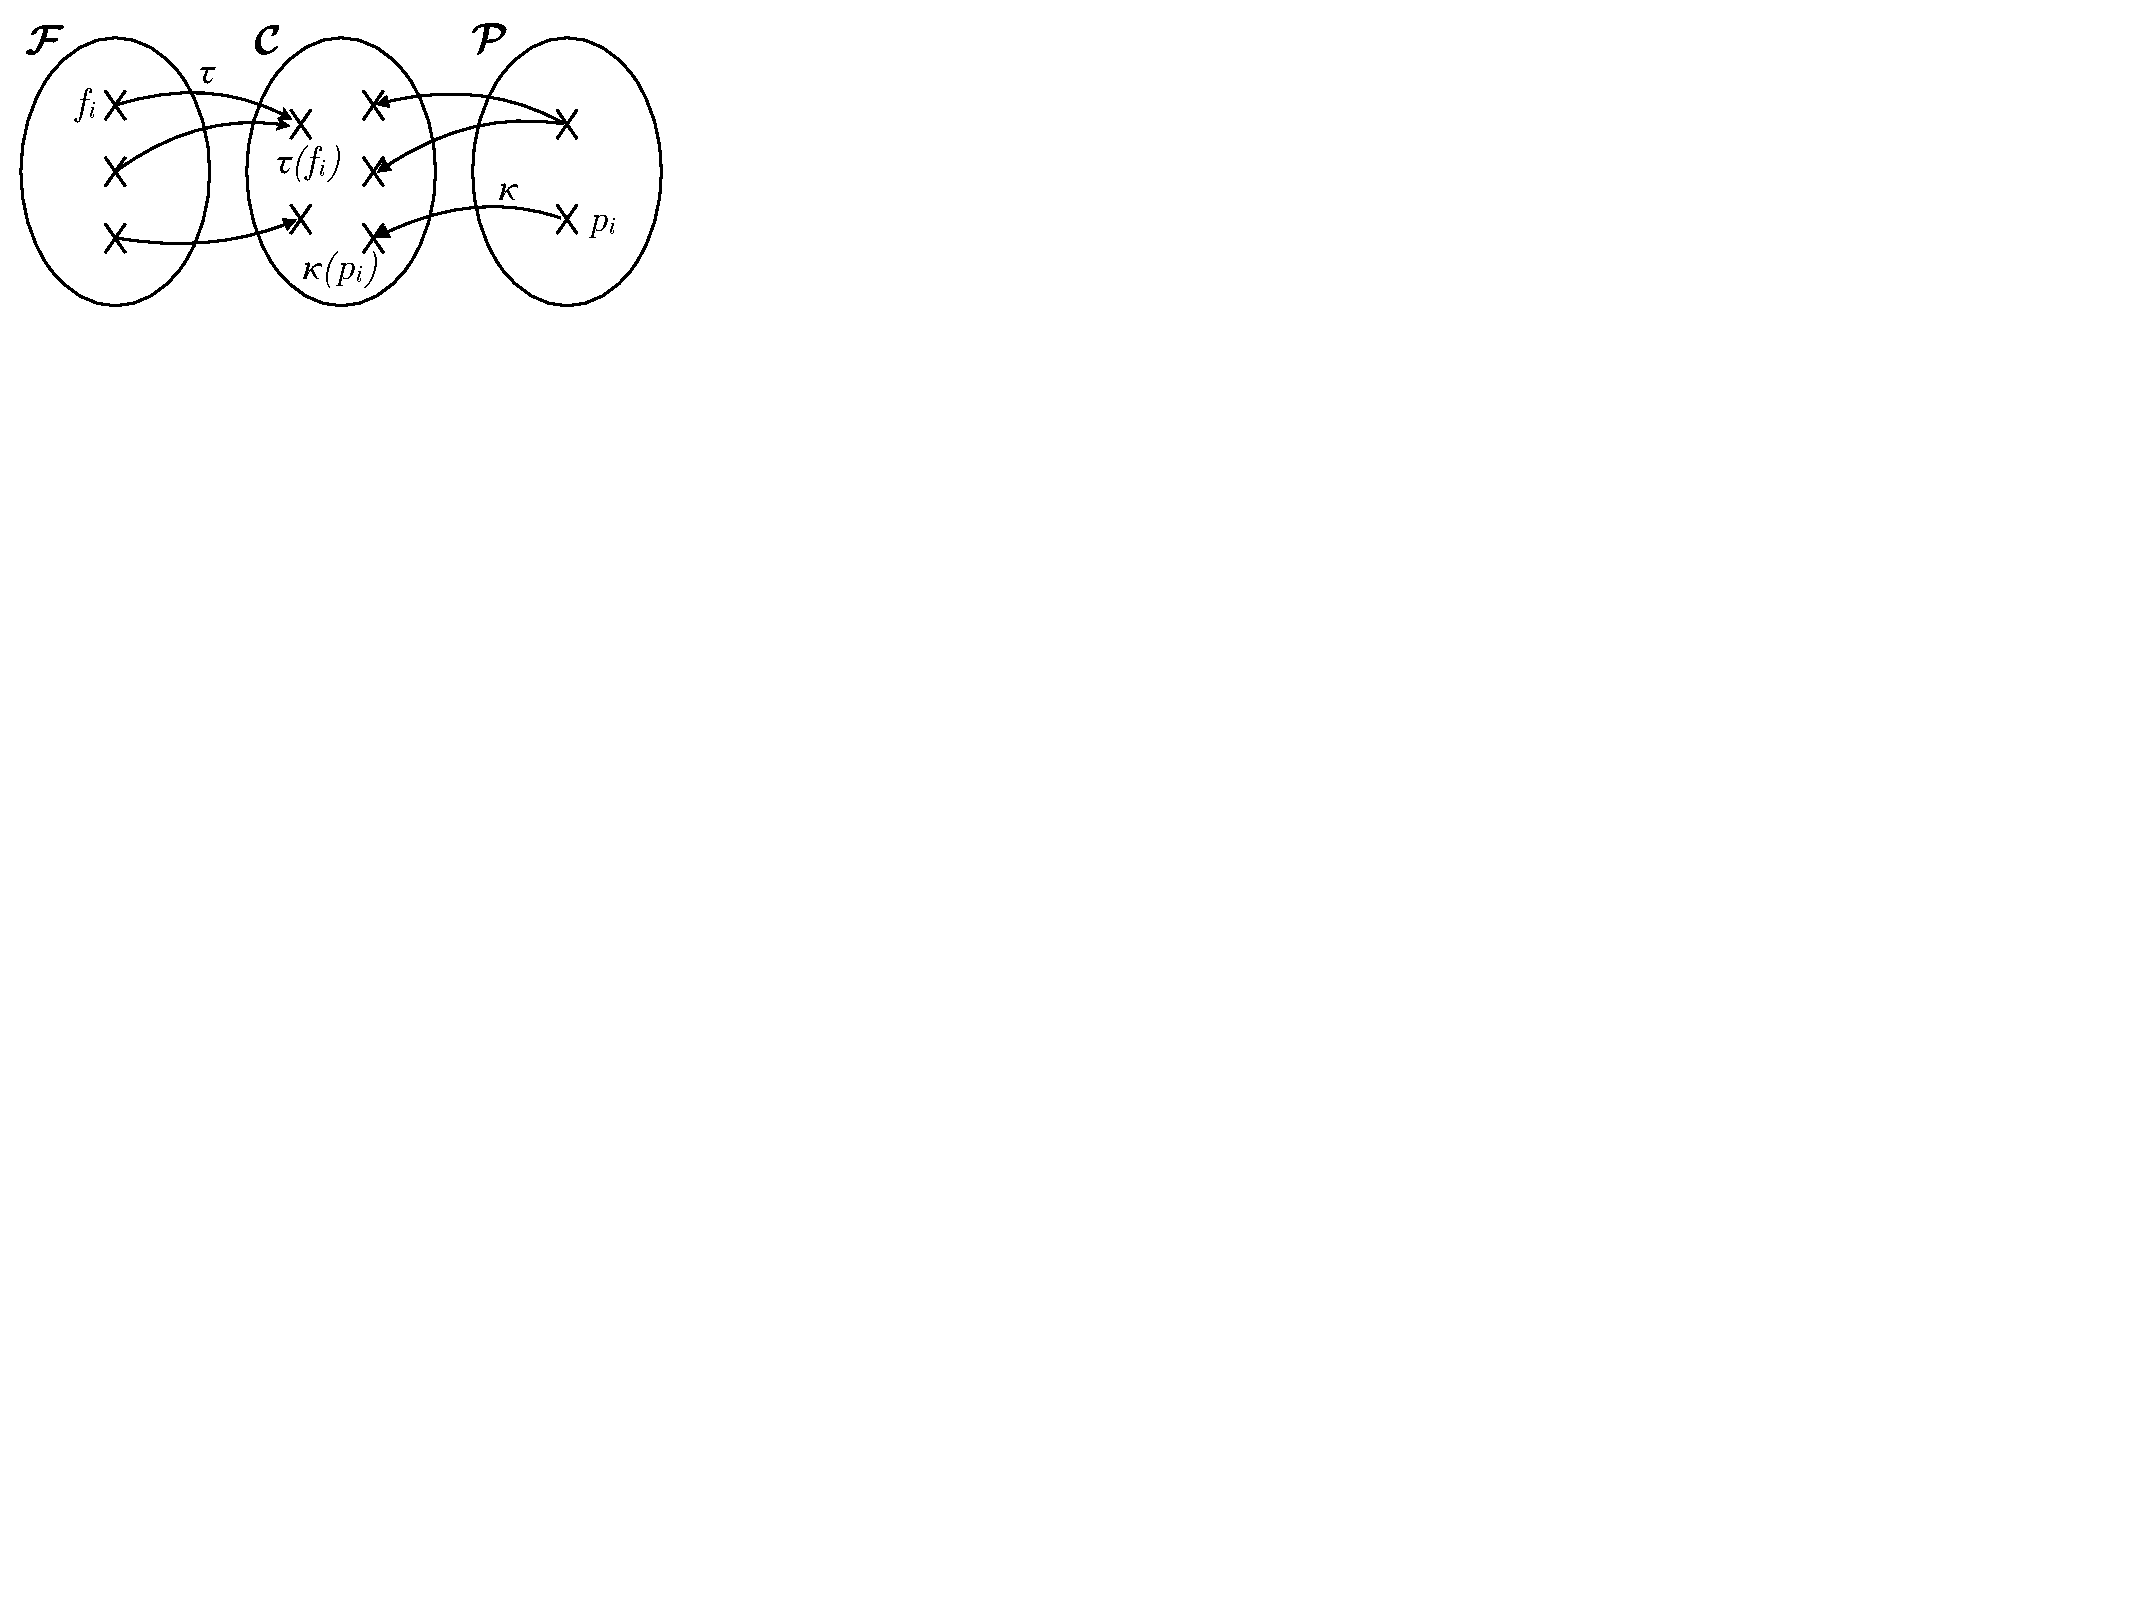
\includegraphics[clip, trim=0in 8.5in 9.8in 0in, width=2in]{figures/function-spaces.pdf}
    \vspace{-2mm}
    \caption{The spaces $\mathcal{F}$, $\mathcal{P}$ and $\mathcal{C}$ and the mappings between them.}
    \label{fig:function-spaces}
    \vspace{-2mm}
\end{figure}

Since $\tau(f)$ and $\kappa(p)$ are defined in the the same space $\mathcal{C}$, as a point and as a set of points respectively, one can compare $\tau(f)$ with each element in $\kappa(p)$, to see if the load can be "covered" by a capability, resulting in our basic capacity theorem: that if $\exists\ c \in \kappa(p) \geq \tau(f), f \rightrightharpoons p$.

%Finally, we define a set of operators which act on $\mathcal{C}$ that calculate the joint characteristic functions of composed functions and networks of pipelines from their constituent functions and pipelines' characteristic functions, extending our embedding theorem to multi-pipeline networks and multi-function programs.

\subsection{Characteristic Functions}
% To determine if an $f$ is embeddable into a $p$, we require a way of comparing $f$ and $p$. XX $f$ and $p$, however, have very different formats, making side by side comparison highly unintuitive. The key insight that makes such comparison possible is that we can ...

%is that both $f$ and $p$ represent computations. The main contribution of this paper is that we can find a common characterization for these computations, which we define using the notion of characterization functions.

% Our characterization function extracts the key properties of a computation (routing functions) or computational capacity (pipelines) in a form that permits comparison. Surprisingly, these properties are simply the domain $dom(M)$ and range $range(M)$ for every subset $M$ of the set of match fields. 

% \begin{definition}
% The {\em domain $dom(M)$} of a subset $M$ of match fields is the set of values ... can take.
% \end{definition}

% \begin{definition}
% The {\em range $range(M)$} of ... is the set of values of a subset $M$ of match fields that can be distinguished.
% \end{definition}

% Domain and range can take any positive integer or a special value, $\intercal$, treated as positive infinity, which denotes a field whose value can be ignored. 

We begin by defining a generic characteristic function $c$.
\begin{definition} A {\em characteristic function $c$} is a mapping from each subset $M$ of a packet's match fields to a vector consisting of two components: 
\begin{equation*}
c(M) \overset{\Delta}{=} <scope(M),\ ec(M)>.
\end{equation*}
\end{definition}

%\yry{fix} 
We refer to the two components of $c(M)$'s vector as $c(M)[scope]$ and $c(M)[ec]$ respectively.


%Suprisingly, these properties are simply the domain and a property we denote \textit{f-equivalence class number} of every subset of a computation's inputs $M \in 2^\mathcal{M}$. 

%We will offer intuition into the behavior of these properties when we define mappings from $\mathcal{F}$ and $\mathcal{P}$ to $\mathcal{C}$. For now it suffices to state that these properties' values can be positive integers or a special value, $\top$, which we interpret as positive infinity, and thus our characteristic function is simply the mapping:

%\begin{equation}
%c : 2^\mathcal{M} \rightarrow (\mathbb{N} + \{\top \})^2\\
%\end{equation}

%We use our mapping to define a partial order over $\mathcal{C}$ by equipping $\mathcal{C}$ with the comparator:

%, we define a comparator over $\mathcal{C}$. Our comparator equips $\mathcal{C}$ with a partial order. 
Given two characteristic functions, one can compare them. 

\begin{definition}We define {\em $c_i$ dominates $c_j$}, denoted as $c_i \geq c_j$ as follows:
\begin{equation*}
\begin{split}
c_i \geq c_j \overset{\Delta}{=}\ \forall\ n \in\ &\{scope, ec\},\\
&\forall\ M \in 2^\mathcal{M},\ c_i(M)[n] \geq c_j(M)[n].
\end{split}
\end{equation*}
\end{definition}

To verify our capacity theorem, we need to compare a set of characteristic functions with a single characteristic function.

%Below we need ..., we define a comparator $\trianglerighteq$ between a $C \in 2^\mathcal{C}$ and a $c \in \mathcal{C}$ from Definition~\ref{def:comparator}.

\begin{definition}
A set of characteristic functions $C_i$ {\em dominates} a characteristic function $c_j$, denoted as $C_i \trianglerighteq c_j$, if a $c_i \in C_i$ dominates $c_j$:

\begin{equation*}
C_i \trianglerighteq c_j \overset{\Delta}{=} \exists\ c_i \in C_i : c_i \geq c_j.
\end{equation*}
\end{definition}
 
\subsection{Characterization of a Routing Function} 
Given the concept of characteristic functions, we now derive the characteristic function, denoted as $\tau(f)$, of a routing function $f$. 

\begin{definition}
\label{def:set-comparator}
The {\em scope} of the characteristic function of a routing function for a subset of packet match fields $M$ is the size of the domain of valid values of $M$:
\begin{equation*}
\tau(f)(M)[scope] \overset{\Delta}{=} dom(M)
\end{equation*}
\end{definition}

$\tau(f)(M)[ec]$ is a property that we build from the concept of f-equivalence: 
%We define f-equivalence $\sim_f$ as a binary property between values of $M$ which denotes that these values cannot be distinguished by $f$. We formalize it as follows:
\begin{definition} We define {\em f-equivalence}, denoted as $\sim_f$, as a relationship between two values of $M$, which we write as $v_i(M)$ and $v_j(M)$, which denotes that these values cannot be distinguished by $f$:
\begin{equation*}
\begin{split}
&v_i(M) \sim_f v_j(M) \overset{\Delta}{=} \forall\ v_k(\mathcal{M} - M) \in dom(\mathcal{M} - M),\\
&\qquad f(v_i(M), v_k(\mathcal{M} - M)) = f(v_j(M), v_k(\mathcal{M} - M)). 
\end{split}
\end{equation*}
\end{definition}

%A characteristic function maps each $M$ to xxx. For a routing function, compute the mapping in x way.  ...the proceed to define our mapping, denoted $\tau_e$, from a routing $f \in \mathcal{F}$ to its characteristic function $c \in \mathcal{C}$. We start by defining the properties, domain and equivalence class number, that a $c$ maps $\forall\ M \in 2^M$ to in the context of an $f$.

%The domain of a f's $M$ $dom(M)$, as we defined in our model of $f$, is simply the set of values of $M$ permitted by $f$. 

%The f-equivalence class number of an $f$'s $M$ is rooted in our concept of f-equivalence, $\sim_f$. f-equivalance is a binary property of values of $M$, $v_i(M) \sim_f v_j(M)$, and intuitively means that $v_i(M)$ and $v_j(M)$ are not distinguished by $f$, or more formally: 

%\begin{equation}
%\begin{split}
%v_i(&M) \sim_f v_j(M) \triangleq f(v_i(M), v_k(\mathcal{M} - M)) = \\ 
%&f(v_j(M), v_k(\mathcal{M} - M))\ \forall\ v_k(\mathcal{M} - M) \in dom(%\mathcal{M} - M)
%\end{split}
%\end{equation}

Our definition of f-equivalence leads naturally to our definition of an f-equivalence class. 
\begin{definition} An {\em f-equivalence class}, denoted as $[v_i(M)]_f$, is the set of all values f-equivalent to a given $M$'s value $v_i(M)$:
\begin{equation*}
[v_i(M)]_f \overset{\Delta}{=} \{v_j(M) \in dom(M) : v_i(M) \sim_f v_j(M)\}.
\end{equation*}
\end{definition}

Counting equivalence classes gives us the concept of f-equivalence class number.
 
\begin{definition}
The {\em f-equivalence class number} of $M$, denoted as $|dom(M)/\sim_f|$, is the cardinality of $M$'s set of f-equivalence classes. 
\end{definition}

We now arrive at our definition of $\tau(f)(M)[ec]$.

\begin{definition} The {\em ec} of a routing function's characteristic function for an $M$ is the cardinality of $M$'s set of f-equivalence classes: 
\begin{equation*}
\tau(f)(M)[ec] \overset{\Delta}{=} |dom(M)/\sim_f|
\end{equation*}
\end{definition}
%Given these definitions, we define the characteristic function $\tau(f)$ of an $f \in \mathcal{F}$ as:

% to its characteristic function $c \in \mathcal{C}$.

\begin{definition} {\em The characteristic function $\tau(f)$ of a routing function} characterizes $f$'s computational load:
\begin{equation*}
\tau(f)(M) \overset{\Delta}{=} (dom(M),\ |dom(M)/\sim_f|).
\end{equation*}
\end{definition}


%of $M$ is therefore simply the cardinality of the set of its f-equivalence classes, $|dom(M)/\sim_f|$.

%Our mapping from $f \in \mathcal{F}$ to their characteristic functions $\tau_e$ proceeds straightforwardsly from our definitions of domain and f-equivalence class number:

%\begin{equation}
%\begin{split}
%&\tau_e : \mathcal{F} \rightarrow \mathcal{C}\\
%&f \mapsto c : c(M) =(dom(M),|dom(M)/\sim_f|)\ \forall\ M \in 2^M
%\end{split}                   
%\end{equation}

While $\tau(f)$ is powerful it is impractical because f-equivalence class number is costly to directly calculate. We therefore bound a $\tau(f)$ by defining the bounding characteristic function of a routing function $\tau_G(f)$ which is easily derivable from $f$'s DFG. This function characterizes an upper bound on $f$'s computation load: $\tau_G(f)$ dominates $\tau(f)$.

We find $\tau_G(f)[scope]$ as before. Instead of calculating $\tau_G(f)[ec]$, however, we determine an upper bound for with the value of specific vertex cut in $G_f$, $f$'s DFG. We now construct this cut.

%Before we transform a routing function into a DFG we apply two key transformations. First, we enforce single state assignment, by breaking up and renaming multiply-assigned variables. Second, we replace if statements with guard variables, transforming control dependencies into data dependencies. For example, \texttt{L3} and \texttt{L4} of \texttt{onPkt} would be transformed from:
%\begin{verbatim}
%L3: if (verify(srcPort, srcIP)):
%L4:   dstCond = condTbl[dstIP, dstPort]
%\end{verbatim}

%to:
%\begin{verbatim}
%L3: g0 = verify(srcPort, srcIP)):
%L4: if g0: dstCond = condTbl[dstIP, dstPort]
%\end{verbatim}

%Given these transformations, we now define the concept of a DFG.

%\begin{definition}
%A DFG $G_f = (V_f, E_f)$ of a $f$ is a vertex weighted dag corresponding to a function such that: $V_f$ is the set of variables in a SSA $f$, the weights of a variable in $V_f$ is its domain size, and $E_f$ is a set of directed edges such that there is a directed edge between two variables if the source variable appears in the target variable's assignment.
%\end{definition}

%We now define a particular type of min-cut in a function's DFG.

%Specifically, we calculate $\tau_G(f)[ec]$ using a vertex min-cut we define below:
\begin{definition} Let $V_f(M)$ be the vertices of $m_i \in M$ in $G_f$, and $D_f(M)$ be the vertices in $G_f$ descended from $V_f(M)$. 
\vspace{2mm}

The {\em vertex-min-cut of $M$}, $G_f.vertexMinCut(M)$, is the product of the weights of the vertices in the minimum weight vertex cut severing $V_f(M)$ from $D_f(\mathcal{M} -M)$.
\end{definition}

%We have arrived at our definition of $\tau(f)[ec]$.

%\begin{definition} $\tau(f)(M)[ec] \overset{\Delta}{=} G_f.vertexMinCut(M)$ is the minimum weight set of vertices severing $V_f(M)$ from $D_f(M)$, and is a bound on $\tau_e(f)(M)[ec]$
%\end{definition}

Given this cut, we define $\tau_G(f)$ follows:

%Let $V_f(M)$ be the set of vertices in $G_f$ that represent $m_i \in M$ and $D_f(M)$ be the set of vertices in $G_f$ descended from $V_f(M)$. Then the range of an $f$'s characteristic function is $G_f.vertexMinCut(V_f(M),\ D_f(M))$.

%Given this concept, $\tau$, our second mapping from a routing function to its characteristic function is:

\begin{definition} {\em The characteristic function $\tau_G(f)$ of a routing function} characterizes an upper bound on $f$'s computational load; $\tau_G(f)$ dominates $\tau(f)$:
\begin{equation*}
\tau_G(f)(M) \overset{\Delta}{=} (dom(M),\ G_f.vertexMinCut(M)).
\end{equation*}
\end{definition}

\para{Example:} We illustrate these concepts with our example routing function \texttt{onPkt}.

Consider \texttt{onPkt}'s match fields \texttt{srcIP} and \texttt{srcPort}. Each are only read once: on \texttt{L3}, by the boolean function \texttt{isVerified}. Thus, while \texttt{srcIP} and \texttt{srcPort} may have many f-equivalence classes individually, (\texttt{srcIP}, \texttt{srcPort}) only has two: values that \texttt{isVerified} evaluates to $0$, and values it evaluates as $1$.

Suppose \texttt{onPkt} is a routing function for a small commercial network fronted by a NAT with $50$ hosts each running a limited set of applications that only use $200$ standard ports. Given this, $dom(\texttt{srcIP}, \texttt{srcPort}) = 10000$, and thus $\tau(\texttt{onPkt})(\texttt{srcIP}, \texttt{srcPort}) = (10000, 2)$. 

While the equivalence class number of (\texttt{srcIP}, \texttt{srcPort}) was straightforwards, the equivalence class number of most other subsets of \texttt{onPkt}'s inputs is not so obvious. We therefore bound $\tau(\texttt{onPkt})$ with $\tau_G(\texttt{onPkt})$, which we calculate using \texttt{onPkt}'s DFG $G_{\texttt{onPkt}}$, shown in Fig.~\ref{fig:onpkt-dfg}.

%While finding the equivalence class number of (\texttt{srcIP}, \texttt{srcPort}) is straightforwards, the number of equivalence classes of other subsets of \texttt{onPkt}'s inputs such as (\texttt{srcIP}, \texttt{srcPort}, \texttt{dstIP}) is less obvious, making it difficult to calculate $c_{e,\texttt{onPkt}}$. Fortunately, we can calculate $c_{\texttt{onPkt}}$ more simply by generating \texttt{onPkt}'s DFG $G_{\texttt{onPkt}}$, shown in Fig.~\ref{fig:onpkt-dfg}.

\begin{figure}[tbh]
    \centering
    \vspace{-1mm}
    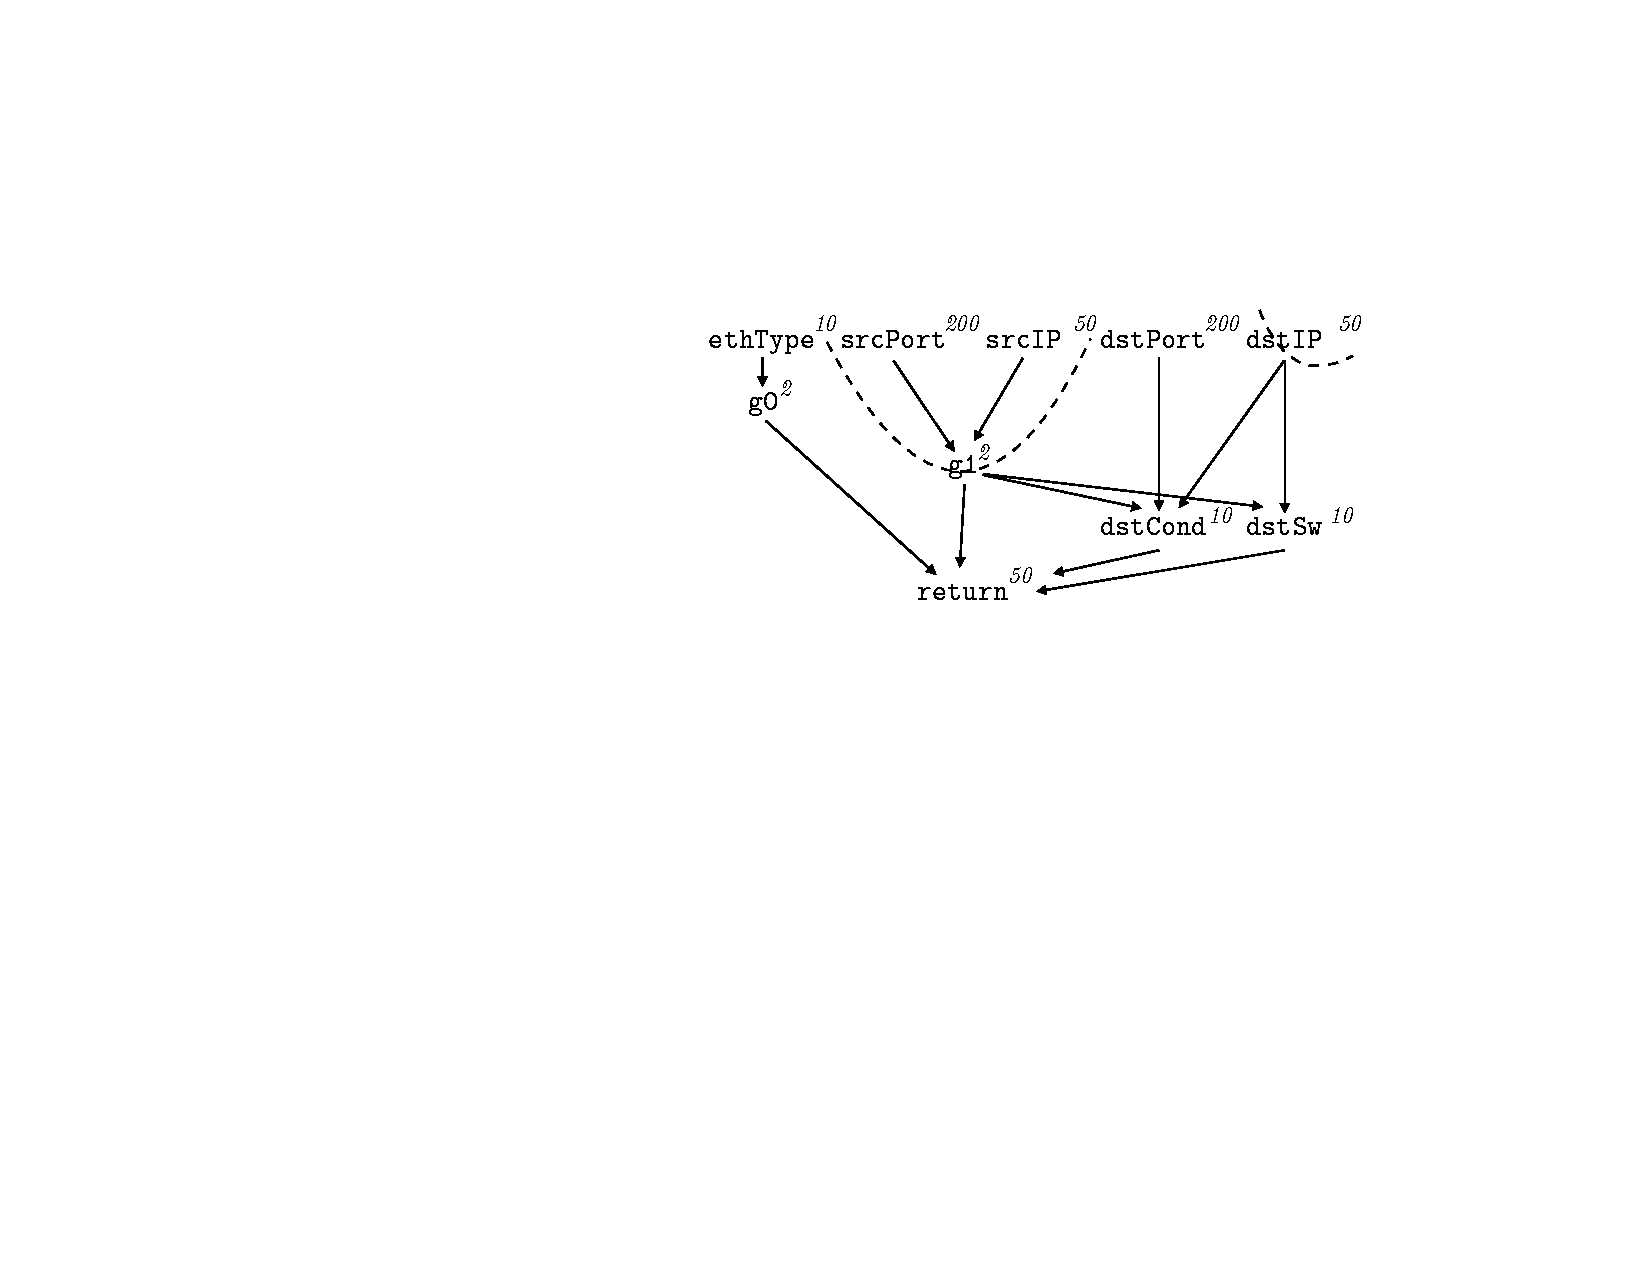
\includegraphics[scale = 0.6]{figures/figure5.pdf}
    \vspace{-2mm}
    \caption{The routing function \texttt{onPkt}'s DFG $G_{\texttt{onPkt}}$ and the cut $(\texttt{srcIP}, \texttt{srcPort}, \texttt{dstPort})$.}
    \label{fig:onpkt-dfg}
    \vspace{-2mm}
\end{figure}

%In $G_{\texttt{onPkt}}$, vertices such as \texttt{dstSw} correspond to \texttt{onPkt}'s variables, edges such as (\texttt{dstIP}, \texttt{dstSw}) imply that the source vertex \texttt{dstIP} is used in the target vertex \texttt{dstSw}'s assignment, and vertex weights such as $w(\texttt{srcIP}) = 50$ indicate their vertices' domain.

To bound, for example, the equivalence class number of \texttt{onPkt}'s inputs (\texttt{srcIP}, \texttt{srcPort}, \texttt{dstIP}) we take the vertex-min-cut in $G_\texttt{onPkt}$ between their vertices and every vertex descended from \texttt{onPkt}'s other inputs: (\texttt{ethType}, \texttt{dstPort},\texttt{g0}, \texttt{dstCond}, \texttt{return}). This vertex-min-cut is indicated in Fig.~\ref{fig:onpkt-dfg} by a dotted line.

%In $G_{\texttt{onPkt}}$, $G_{\texttt{onPkt}}.vertexMinCut(($\texttt{srcIP}, \texttt{srcPort}, \texttt{dstIP}$))$ is the product of vertex min cut weights between (\texttt{srcIP}, \texttt{srcPort}, \texttt{dstIP}) and the set of vertices descended from the remainder of \texttt{onPkt}'s inputs (\texttt{ethType}, \texttt{dstPort}): (\texttt{ethType}, \texttt{dstPort}, \texttt{g0}, \texttt{dstCond}, \texttt{return}), indicated by the dotted line in Fig.~\ref{fig:onpkt-dfg}. 

The vertices in this cut, (\texttt{g1}, \texttt{dstIP}) have weight $50$ and $2$, and thus $\tau_G(\texttt{srcIP}, \texttt{srcPort}, \texttt{dstIP}) = (50000,\ 100)$.


%The vertices in (\texttt{srcIP}, \texttt{srcPort}, \texttt{dstIP})'s vertex-min-cut are: (\texttt{g1}, \texttt{dstIP}) which have weight $50$ and $2$ respectively, and thus we find $100$ as an bound on this subset's number of equivalence classes. This implies that $c_\texttt{onPkt}(\texttt{srcIP}, \texttt{srcPort}, \texttt{dstIP}) = (50000,\ 100)$.

%he set of verticies in $G_f$ that represent $m_i \in M$ be $V_f(M)$

%Unfortunately, while $\tau_e$ is powerful, f-equivalence class number is costly to directly calculate and difficult to work with. Thus, in practice, we approximate $\tau_e$ with a second mapping from $\mathcal{F}$ to $\mathcal{C}$, $\tau$.

%The key insight underlying $\tau$ is that we can approximate f-equivalence class number using an $f$'s DFG, $G_f = (V_f, E_f)$. An $f$'s DFG is... \cleet{TODO: Define DFG}

%Given our description of an $f$'s DFG, our approximation for f-equivalence class number quickly follows. If the set of vertices in $V_f$ that represent a given $M$ is $V_f(M)$ and the set of vertices in $V_f$ descended from $V_f(M)$ is $D_f(M)$, we can approximate $|dom(M)/\sim_f|$ as the vertex min-cut separating $D_f(M)$ from $V_f(M)$ (which may include vertices in $V_f(M)$), which we denote as: $G_f.vertexMinCut(V_f(M),\ D_f(M))$. Substituting this approximation for $M$'s equivalence class number into $\tau_e$ yields $\tau$:

%\begin{equation}
%\begin{split}
%&\tau : \mathcal{F} \rightarrow \mathcal{C}\\
%&f \mapsto c : c(M) = (dom(M),\\
%&\qquad G_f.vertexMinCut(V_f(M),\ D_f(M))\ \forall\ M \in 2^M
%\end{split}                   
%\end{equation}

%\para{Example:} \cleet{TODO: Add example}

%....The first component of We begin by noting that routing functions can be very complex. Such functions may employ arbitrary computation to generate arbitrary mappings between the space of all packet header values and the space of all routing actions. Such spaces, furthermore, may be large. An IPv6 header alone, for example, contains 40 bytes of information, and typical routing functions increasingly read multiple headers spanning multiple layers of the internet stack. Our main result collapses this complexity, distilling routing functions down to their essential information transmission requirements.


%We begin by introducing the notion of f-equivalence, which we will use to parameterize $f$ transmission requirements.
%\vspace{1mm}

%\noindent \textsc{Definition 1 - f-equivalence:} An $S \in 2^M$'s values $u$ and $v$ are f-equivalent iff $f(S = u, M-S) = f(S = v, M-S)\ \forall$ values of $ M-S$.
%\vspace{1mm}

%Our definition of f-equivalence leads naturally to the definition of a f-equivalence class:
%\vspace{1mm}

%\noindent \textsc{Definition 2 - f-equivalence classes:} A set of mutually f-equivalence values of an $S$.
%\vspace{1mm}

%Before continuing, we provide the reader with some intuition into how f-equivalence classes behave. Consider the $f$ \texttt{onPkt}, below:

%\begin{verbatim}
%def onPkt(Addr dstIP, Port dstPort):
%  if dstPort <= 1024:
%    egress = stdHostTbl[dstIP]
%  elif dstPort == 1025:
%    egress = usrHostTbl[dstIP]
%  else:
%    return Drop();
%  return Forward(egress);
%\end{verbatim}

%The domain of \texttt{onPkt}'s input \texttt{dstPort} is $2^{16}$, since the TCP protocol allows TCP sockets to take any port number between $0$ and $65535$. However, \texttt{onPkt} only depends very particularly on where \texttt{dstPort}'s value falls within this domain, specifically on whether \texttt{dstPort} is $\leq 1024$, $1025$, or $> 1025$. Regardless of the value of \texttt{dstIP}, \texttt{onPkt} will always output the same result for any values of \texttt{dstPort} in the same set. Thus, we say that values within these sets are equivalent, and that the sets themselves comprise \texttt{onPkt}'s equivalence classes.

%We use our definition of f-equivalence classes to define the central abstraction of our theorem: the header set equivalence class function $h$, which associates every $S \in 2^M$ with a number of f-equivalence classes.
%\vspace{1mm}

%\yry{Move to early}
%\noindent \textsc{Definition 3 - Header f-equivalence class function:} A mapping $h$ from $\forall\ S \in 2^M$ to a number of f-equivalence classes, $2^M \rightarrow \mathbb{N}$.
%\vspace{1mm}

%\noindent \textsc{Definition 4 - Header f-equivalence class function space:} The space of $\forall\ h$, $H$.
%\vspace{1mm}

%The space $H$ is a powerful space to consider because we can define a mapping from $\forall\ f \in F$ to exactly one $h \in H$, $\tau$, which we illustrate in Fig.~\ref{fig:function-spaces}. and define below:
%\vspace{1mm}


%\noindent \textsc{Definition 5 - Function header f-equivalence class map, $\tau$:} $\tau$ is a mapping $f \rightarrow h$, \textit{s.t.} $h(S)$ is $S$'s number of f-equivalence classes $\in f$.
%\vspace{1mm}

\subsection{Characterization of a Pipeline}
We now define $\kappa(p)$, the set of characteristic functions of a pipeline $p$. We start by defining a path $\rho$ through a pipeline $p$.

%\noindent{\em Overview}:??

\begin{definition}
A path, $\rho$, in a $p$ is a path through $p$'s dag $\langle t_1, ..., t_n \rangle$ such that $t_1$ is a root table and $t_n$ an egress table in the $p$.
\end{definition}

As an example, \exampledp\ contains two paths: $\langle \texttt{t1}, \texttt{t2}, \texttt{t3}, \texttt{t4}, \texttt{t5} \rangle$, and $\langle \texttt{t1}, \texttt{t6} \rangle$, which we denote as $\rho_{L2}$ and $\rho_{L3}$ respectively. 

We define, $\forall\ \rho \in p,\ \kappa_\rho(p)$ as the characteristic function of the a path through a pipeline. 

\begin{definition} {\em The characteristic function set $\kappa(p)$} of a $p$ is the union of $\forall\ \rho \in p$'s characteristic functions:
\begin{equation*}
\kappa(p)(M) \overset{\Delta}{=} \{c \in \mathcal{C} : c = \kappa_\rho(\rho)\ \forall\ \rho \in p\}.
\end{equation*}
\end{definition}

We now construct the characteristic function of a path $\rho$ by introducing the following definitions:

%Given these definitions, we arrive at $\kappa_\rho(\rho)$, the characteristic function of a $\rho$.

%Each $\rho$ has a characteristic function where $dom(M)$ is the maximum number of values of $M$ that $\rho$ can read and $range(M)$ is the maximum number of equivalence classes of $M$ $\rho$ can distinguish. We determine the values of $dom(M)$ and $range(M)$ by introducing the following definitions:

%First, we define the input closure $\bar{M}_\rho(t_i)$ of a $t_i$ in $\rho$ as:

\begin{definition} The {\em input closure $\bar{M}_\rho(t_i)$} of a table $t_i \in \rho$ is the set of inputs that $t_i$ can obtain information about:
\begin{equation*}
\begin{split}
\bar{M}_\rho(t_i) \overset{\Delta}{=} \{m_i \in \mathcal{M} :\ &m_i \in I(t_i)\ \vee\\ &m_i \in \bar{M}_\rho(t_j)\ s.t.\ r(t_j) \in I(t_i)\}.
\end{split}
\end{equation*}
\end{definition}

%Next, we define the closure set, $\bar{\bar{M}}_\rho(M)$ of a $\rho$ as:
\begin{definition} The {\em closure set, $\bar{\bar{M}}_\rho(M)$} of a $\rho$'s $M$ is the set of $t_i \in \rho$ with input closure $M$.
\begin{equation*}
\bar{\bar{M}}_\rho(M) \overset{\Delta}{=} \{t_i \in \rho : \bar{M}_\rho(t_i) = M\}. 
\end{equation*}
\end{definition}

Using these definitions, we define the characteristic function of a $\rho$ as:
\begin{definition} {\em The characteristic function $\kappa_\rho(\rho)$ of a $\rho$} characterizes the computational capacity of a $\rho$. 

$\kappa_\rho(\rho)[scope]$ is the maximum number of values of $M$ that $\rho$ can read and $\kappa_\rho(\rho)[ec]$ is the maximum number of equivalence classes of $M$ that $\rho$ can distinguish.

\begin{equation*}
\begin{split}
&\kappa_\rho(\rho)(M) \overset{\Delta}{=}\\
&\begin{cases}
\bar{\bar{M}}_\rho(M) \neq \emptyset \quad \quad (min[maxrules(t_i) : t_i \in \bar{\bar{M}}_\rho(M)],\\
\quad \quad \quad \quad \quad \quad \quad \quad  min[2^{bits(r(t_i))} : t_i \in \bar{\bar{M}}_\rho(M)])\\
\bar{\bar{M}}_\rho(M) = \emptyset \wedge \exists\ m_i \in M :\\
m_i \notin \bigcup_{t_i \in \rho} \bar{M}(t_i, \rho)\  \quad \quad \quad \quad \quad (1, 1)\\
otherwise, \quad \quad \quad \quad \quad \quad \quad \ \ \ \ \, \, \,  (\intercal, \intercal).
\end{cases}
\end{split}
\end{equation*}
\end{definition}

\para{Example:} As before, we provide intuition into the characteristic functions of pipelines using our example pipeline \exampledp.

Recall from our model that \exampledp{} contains two $\rho$: $\rho_{\texttt{L2}}$ and $\rho_{\texttt{L3}}$. Consider the table \texttt{t4}, only contained by $\rho_{\texttt{L3}}$. The input closure $\bar{M}_{\rho_{\texttt{L3}}}(\texttt{t4})$ is (\texttt{srcIP}, \texttt{srcPort}, \texttt{dstIP}) since \texttt{t4} reads \texttt{dstIP} and \texttt{r(t2)}, and \texttt{t2} in turn reads \texttt{srcIP} and \texttt{srcPort}. The closure set, $\bar{\bar{M}}_{\rho_\texttt{L3}}(\texttt{srcIP}, \texttt{srcPort}, \texttt{dstIP})$, of \texttt{t4}'s inputs in $\rho_{\texttt{L3}}$ is $\{\texttt{t4}\}$: \texttt{t4}'s input closure is unique.

Thus, $\kappa_{\rho_{\texttt{L3}}}(\bar{M}_{\rho_{\texttt{L3}}})$ $=$ $\kappa_{\rho_{\texttt{L3}}}(\texttt{srcIP}, \texttt{srcPort}, \texttt{dstIP})$ $=$ $(maxRules(\texttt{t4}),$ $2^{bits(r(\texttt{t4}))})$. In the case that \texttt{t4} has $2^{20}$ rules and a $16$ bit output register, $\kappa_{\rho_{\texttt{L3}}}(\bar{M}_{\rho_{\texttt{L3}}}) = (2^{20}, 2^{16})$.

Further, consider the subset of \exampledp's match fields $(\texttt{srcMac},\ \texttt{dstMac})$. $\rho_{\texttt{L3}}$ does not contain the inputs \texttt{srcMac} or \texttt{dstMac} and thus it can only realize functions that contain them in the unlikely event that all are constants.  Constants have domain $1$ and $1$ equivalence class. Thus the value of $\kappa_{\rho_{\texttt{L3}}}$ for any set of outputs containing \texttt{srcMac} is $(1, 1)$.

Finally, consider the subset of \exampledp's match fields $(\texttt{srcIP},\ \texttt{srcPort})$. \texttt{srcIP} and \texttt{srcPort} are both read by $\rho_{\texttt{L3}}$, but $(\texttt{srcIP},\ \texttt{srcPort})$ is not an input closure of any $t_i \in \rho_{\texttt{L3}}$. In this case, it is not necessary to consider $(\texttt{srcIP},\ \texttt{srcPort})$ to verify realizability, and thus $\kappa_{\rho_{\texttt{L3}}}(\texttt{srcIP},\ \texttt{srcPort}) = (\intercal, \intercal)$, indicating that we can skip this field during comparison with a routing funciton's $\tau$.

%\qquad min[\{2^{r(t_i)} : t_i \in T_j\}]\\


%Specifically, we define a path $\rho$ in a $p$ as a path through $p$'s dag $\langle t_1, ..., t_n \rangle$ such that $t_1$ is $p$'s root and $t_n$ is an egress table. To define the char functions for $\rho$, we introduce a few definitions.

%Define the input closure of a table ti in $\rho$: 
%\begin{definition}[Input closure]

%\end{definition}

%Define the matched tables of $\rho$: 
%\begin{definition}[Matched tables]

%\end{definition}


%With the defi
% and we denote the mapping from each $\rho \in p$ to its characteristic function as $k_\rho$.

%[..., define the concept of the char function for each path]. A pipeline is chara. by the function of a routing funtion $f$.  We now define our mapping from $p \in \mathcal{P}$ to $C \in 2^{\mathcal{C}}$, $\kappa$. 

%We begin by characterizing the set of $c$ that $\kappa$ maps a given $p$ to. The key insight underlying this set is that $p$ may contain multiple branches which match on different $M \in \mathcal{M}$ and thus embed different functions. For example, one of \texttt{swPipeline}'s branches matches on L3 match fields and can therefore embed L3 routing functions, while the other matches on L2 match fields and can embed L2 routing functions. We therefore characterize each path through a $p$'s branches separately.

% We define the characteristic function set a $p$ is mapped to as the set of characteristic functions of $\forall\ \rho \in p$, and therefore $\kappa$ as:

%\begin{equation}
%\begin{split}
%&\kappa : \mathcal{P} \rightarrow  2^\mathcal{C}\\
%&p \mapsto \{c \in \mathcal{C} : c = \kappa_\rho(\rho)\ \forall\ \rho \in p\}
%\end{split}
%\end{equation}

%We now proceed to define the mapping from individual $\rho$ to their characteristic functions, $\kappa_\rho$. As before, we define the properties domain and f-equivalence class number in the context of a $\rho$.

%The domain of a $\rho$'s $M$ is simply the maximum number of values of $M$ that $\rho$ can read. The equivalence class number of $\rho$'s $M$, similarly, is the maximum number of equivalence classes of $M$ $\rho$ can distinguish. 

%These two values are distinct when the $t_i \in \rho$ that read $M$'s output registers are not large enough to contain every equivalence class they can read. For example, if \texttt{swPipeline}'s $t_2$ can contain $2^{16}$ rules but $r(t_2)$ is only $8$ bits, $t_2$ can read $2^{16}$ values of $($\texttt{srcIP}, \texttt{srcPort}$)$, but can only distinguish $2^8$ of their equivalence classes in its output.

%\vspace{1mm}
%\cleet{TODO: Define match field closure}
%\vspace{1mm}

%Given our definitions of domain, equivalence class number and match field closer, we present $\kappa_\rho$ and offer intuition into its mapping.

%\begin{equation}
%\begin{split}
%&\kappa_\rho : \varrho \rightarrow \mathcal{C}\\
%&\rho \mapsto c :\\ 
%&\begin{cases}
%T_j = \{t_i \in \rho : \bar{M}(t_i, \rho) = M\}\\
%T_j \neq \emptyset, c(M) = (min[\{maxRules(t_i) : t_i \in T_j\}],\\
%\qquad min[\{2^{r(t_i)} : t_i \in T_j\}]\\
%\exists\ m_i \in M : m_i \notin \bigcup_{t_i \in \rho} \bar{M}(t_i, \rho),\ c(M) = (1, 1)\\
%otherwise,\ c(m_i) = (\top, \top)
%\end{cases}\\ 
%&\forall\ M \in 2^M
%\end{split}
%\end{equation}

%\cleet{TODO: Offer intuition}

%\begin{equation}
%\bar{M}(t_i, \rho) \triangleq match\ field\ closure\ of\ t_i\ over\ \rho
%\end{equation}

%\begin{equation}
%\bigcup_{t_i \in \rho} \bar{M}(t_i, \rho) \triangleq match\ field\ closure\ of\ \rho
%\end{equation}


%Pipelines can also be very complex. Limiting ourselves to a set of $p$ which read a fixed set of packet fields, $M$, yields an infinite number of $p$ to consider. Even further reducing our scope to $p$ whose number of tables is also fixed still requires us to consider an exponential number of $p$ varying on their control flow links between tables. 

%Surprisingly and beautifully, we can also generate a meaningful mapping between $p \in P$ and a set of $h \in H$, $\kappa$, which too distills $p$ to their essence: the amount of information such a $p$ can carry about its packet fields, which we illustrate in Fig.~\ref{fig:function-spaces}. and define below:
%\vspace{1mm}

%\noindent \textsc{Definition 5 - Pipeline header f-equivalence class map, $\kappa$:} $\kappa$ is a mapping $p \rightarrow $\{h: $h \in H\}$ \textit{s.t.} each $h(S)$ equals  the maximum number of f-equivalence classes of an $f$ that $p$ can compute.
%\vspace{1mm}
%
%Now that we can characterize both $f$ and $p$ with functions $h$ from a unified function space $H$, we define comparators for $h \in H$ to compare $f$ and $p$'s characteristic functions directly.
%\vspace{1mm}
%
%\noindent \textsc{Definition 6 - $h \rightarrow h$ comparator, $>$:} $h_1 > h_2$ iff $h_1(S) > h_2(S)\ \forall\ S$.
%\vspace{1mm}
%
%\noindent \textsc{Definition 7 - $\{h:h \in H\} \rightarrow h$ comparator, $\triangleright$:} $H_1 \triangleright h_2$ iff $\exists\ h_1 \in H_1$ \textit{s.t.} $h_1(S) > h_2(S)\ \forall\ S$.
%\vspace{1mm}%
%
\subsection{Datapath Programming Capacity Theorems}
Combining the preceding definitions to characterize both routing functions and pipelines, we finally arrive at our central result: a sufficient condition for whether a given $f$ can be realized in a given $p$.

\begin{theorem}[Pipeline Realization Theorem] A routing function $f$ can be realized by a pipeline $p$ if $\kappa(p)$, the set of characteristic functions of $p$ dominates $\tau(f)$, the characteristic function of $f$. Formally, we have:
\begin{equation*}
\kappa(p) \trianglerighteq \tau(f) \Rightarrow f \rightrightharpoons p.
\end{equation*}
\end{theorem}

As a corollary, because $\tau_G(f) > \tau(f)$, the Pipeline Realization Theorem extends to $\tau_G(f)$.

\para{Example:} We illustrate our Pipeline Realization Theorem using \texttt{onPkt} and \exampledp. Specifically, our Pipeline Realization Theorem states that $\kappa(\exampledp) \trianglerighteq \tau(\texttt{onPkt}) \Rightarrow \exampledp \rightrightharpoons \texttt{onPkt}$.

Further, $\kappa(\exampledp) \trianglerighteq \tau(\texttt{onPkt})$ is true if $\kappa_\rho(\rho_{\texttt{L2}}) > \tau_G(\texttt{onPkt})$ or $\kappa_\rho(\rho_{\texttt{L3}}) > \tau_G(\texttt{onPkt})$ We verify each conditional by comparing each component of each vector given by each pair of characteristic functions. For example, $\tau(\texttt{onPkt})(\texttt{srcIP},$ $\texttt{srcPort},$ $\texttt{dstIP}$) $ = (50000,\ 100)$,  $\kappa_\rho(\rho_{\texttt{L3}})(\texttt{srcIP},$ $\texttt{srcPort},$ $\texttt{dstIP}$) $ = (2^{20}, 2^{16})$, and thus the input set (\texttt{srcIP}, \texttt{srcPort}, \texttt{dstIP}) does not prevent \texttt{onPkt} from being realized in $\rho_{\texttt{L3}}$.


%By definition~\ref{def:set-comparator}, $c_{\exampledp} \trianglerighteq c_{\texttt{onPkt}} \Leftrightarrow c_{\rho_\texttt{L3}} \trianglerighteq c_{\texttt{onPkt}} \vee c_{\rho_\texttt{L2}} \trianglerighteq c_{\texttt{onPkt}}$. 

%Consider the comparison $c_{\rho_\texttt{L3}} \trianglerighteq c_{\texttt{onPkt}}$. This comparison is true if for each subset of $c_{\rho_\texttt{L3}}$ and $c_{\texttt{onPkt}}$'s inputs $(\texttt{ethType},\ \texttt{srcIP},\ \texttt{srcPort},\ \texttt{dstIP},\ \texttt{dstPort})$ both of $c_{\rho_\texttt{L3}}$'s values are great than $c_{\texttt{onPkt}}$'s.

%For example, recall wthat $c_{\rho_\texttt{L3}}(\texttt{srcIP},$ $\texttt{srcPort},$ $\texttt{dstIP})$ $= (2^{20},\ 2^{16})$ and $c_{\texttt{onPkt}}(\texttt{srcIP},$ $\texttt{srcPort},$ $\texttt{dstIP})$ $=\ (50000,\ 100)$. \yry{rule: do not start a sentence by non-words} $2^{20}$ $>$ $50000$, $2^{16} > 100$, and thus $c_{\rho_\texttt{L3}} > c_{\texttt{onPkt}}$ over this match field subset.

\para{Tightness:} Though the theorem provides only a sufficient condition, tighter results, in particular sufficient and necessary conditions, can be established in multiple settings. In particular, we have the following result:

\begin{definition} A branchless pipeline $p$ is a $p$ whose dag is a path from its root to its output node.
\end{definition}

\begin{theorem} If $p$ is a branchless pipeline, $p$'s table size is large, and each match field $m_i \in \mathcal{M}$ appears in exactly one of $p$'s tables, $\kappa(p) \trianglerighteq \tau_G(f) \Leftrightarrow f \rightrightharpoons p$.
\end{theorem}

%For example, recall that $c_{\rho_\texttt{L3}}(\texttt{srcIP},$ $\texttt{srcPort},$ $\texttt{dstIP})$ $= (2^{20},\ 2^{16})$ and $c_{\texttt{onPkt}}(\texttt{srcIP},$ $\texttt{srcPort},$ $\texttt{dstIP})$ $=\ (50000,\ 100)$. $2^{20}$ $>$ $50000$, $2^{16} > 100$, and thus $c_{\rho_\texttt{L3}} > c_{\texttt{onPkt}}$ over this match field subset.


 In Sec.~\ref{sec:eval1}, we evaluate our realization theorem's tightness on more general pipelines through experiments.

%\para{Multi-function programs:} We now extend our characterization of routing functions to programs of composed functions. We define a binary operator on $\mathcal{C}$, $\bullet_f$, which takes the characteristic functions of two $f$, $\tau(f_i)\ \bullet_f \tau(f_j)$, and computes the characteristic function of their composition $\tau(f_i \bullet f_j)$. The behavior of $\bullet_f$ is undefined on characteristic functions not associated with routing functions. We give $\bullet_f$ below:

%\begin{theorem}
%\begin{equation*}
%\begin{split}
%&\bullet_f :\ \mathcal{C},\ \mathcal{C} \rightarrow \mathcal{C}\\
%&\tau(f_i),\ \tau(f_j) \mapsto c \in \mathcal{C} : c(M) = \\
%&\qquad min[\tau(f_i)(M) + \tau(f_j)(M),\ \tau(f_j)(M \cup \{m_c\})]\\
%&\qquad \forall\ M \in 2^\mathcal{M}
%\end{split}
%\end{equation*}
%\end{theorem}

%\para{Multi-pipeline networks:} Similarly, we extend our characterization of pipelines to networks of multiple composed pipelines by binary operators on $\mathcal{C}$, $+_p$ and $\bullet_p$ which compute the characteristic function sets of two pipelines $p_i$ and $p_j$ composed in parallel and serial respectively. As before, their behavior is undefined on characteristic functions not associated with pipelines.

%\begin{theorem}
%\begin{equation*}
%\begin{split}
%&+_p : \mathcal{C}, \mathcal{C} \rightarrow \mathcal{C} \\
%&\kappa(p_1), \kappa(p_2) \mapsto \kappa(p_1) \cup \kappa(p_2)
%\end{split}
%\end{equation*}
%\end{theorem}

%\begin{theorem}
%\begin{equation*}
%\begin{split}
%&\bullet_p :\ \mathcal{C},\ \mathcal{C} \rightarrow \mathcal{C}\\
%&\kappa(p_i),\ \kappa(p_j) \mapsto c \in \mathcal{C} : c(M) = \\
%&\qquad min[\kappa(p_i)(M) + \kappa(p_j)(M),\\
%&\qquad \qquad \kappa(p_i)(M) + 2^w,\ \kappa(p_j)(M \cup \{m_c\})]\\
%&\qquad \forall\ M \in 2^\mathcal{M}
%\end{split} 
%\end{equation*}
%\end{theorem}

%\subsection{Pipeline embedding algebra}
%In the preceding subsections, we gave our embedding theorems for unlimited and limited size pipelines. In this subsection, we extend these results to multi-pipeline networks and sets of composed functions by defining a capacity algebra to calculate the joint $h$ of composed $f$ and $p$.
